\chapter{Semi-Unsupervised Approach}

Unsupervised methods, consider a human fall as an event that deviate from normality and they are based on one-class classifiers. The main advantage of an unsupervised methods for fall detection is that it can works without knowing any examples related the the class of interest, i.e. the human fall. As aforementioned, this should be the perfect way to go in an application like this, where what we are interested in is very difficult to retrieve or we only have very few data available, but the principal weakness of an unsupervised system is that certain events deviate from normality as the human fall (e.g., the fall of an object), thus they may produce false alarms.
In this Chapter, two types of methods are described: in \secref{sec:user_aided_cin} a OCSVM used-ided method is exposed, while \secref{sec:siamese_few_shot} present an approach based on Siamese neural network for one-shot learning, both of them assessed with samples related to R0 room of the employed dataset \secref{sec:dataset}. An extension of the Siamese approach is presented in \secref{sec:siamese_few_shot} where the entire dataset presented in \secref{sec:dataset} has been used.




\section{A Combined One-Class SVM and Template Matching Approach for User-Aided Human Fall Detection}
\label{sec:user_aided_cin}

The approach proposed here, is the extension of the one presented in \secref{sec:ocsvm_approach} thus, consists of a combined One-Class Support Vector Machine (OCSVM) based method and template-matching classifier that operate in cascade. The template-matching classifier operates in a user-aided supervised manner and it is employed to reduce such errors by using a set of templates that represent these events. Templates are identified by the user that marks the occurrence of a false positive instead of a true human fall event. 
As shown in the previous section, ``unsupervised methods'' are able to overcome the need of manual tuning of ``analytical methods'' and the necessity of a large labelled dataset of ``supervised methods''. In ``unsupervised methods'', falls are discriminated from non-falls based on a model of ``normality'' constructed from a large amount of non-fall events. However, certain events differ from the ``normality'' as human falls, and they may induce the classifier to produce false alarms. As an example, \figref{fig:time_ha} and \figref{fig:spec_ha} show respectively the waveform and the spectrogram of a segment of ``normal'' human activity (footsteps and speech) \figref{fig:time_hf} and \figref{fig:spec_hf} show the waveform and the spectrogram of a segment of human fall, and \figref{fig:time_bf} and \figref{fig:spec_bf} the waveform and the spectrogram of a book fall. The figures show clearly that both falls signals differ significantly from the human activity one, thus a classifier may be induced to consider the fall of a book as the fall of a person.

\begin{figure}[htbp!]
	\centering
	\begin{subfigure}[t]{0.5\columnwidth}
		\centering
		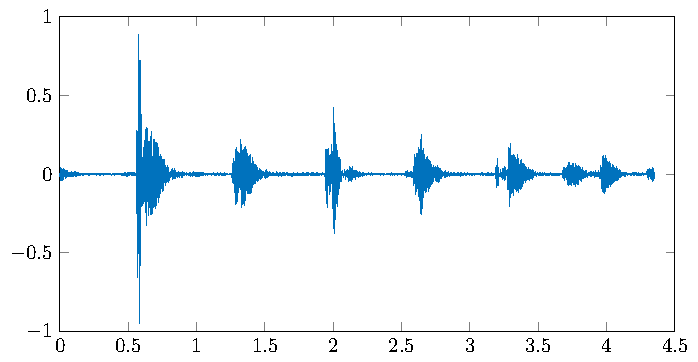
\includegraphics[width=0.9\textwidth]{img/cin/ha_time_.pdf}
		\caption{Normal human activity signal in the time domain.}\label{fig:time_ha}
	\end{subfigure}%
	\begin{subfigure}[t]{0.5\columnwidth}
		\centering
		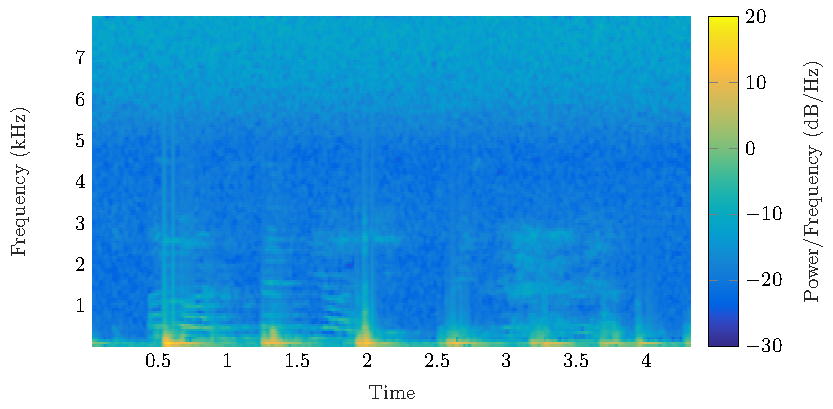
\includegraphics[width=\textwidth]{img/cin/ha_freq_.pdf}
		\caption{Normal human activity signal in the frequency domain.}\label{fig:spec_ha}
	\end{subfigure}
	
	\begin{subfigure}[t]{0.5\columnwidth}
		\centering
		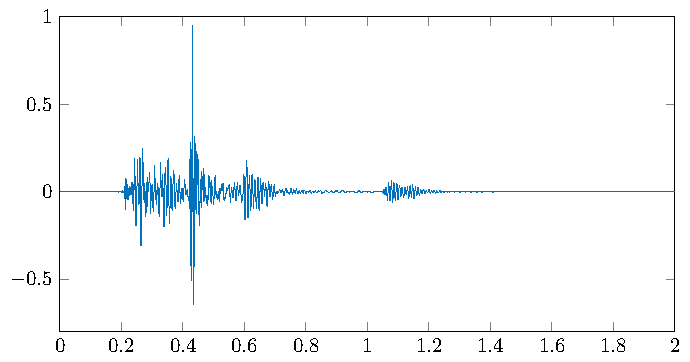
\includegraphics[width=0.9\textwidth]{img/cin/rndy_time_.pdf}
		\caption{Human fall signal in the time domain.}\label{fig:time_hf}
	\end{subfigure}%
	\begin{subfigure}[t]{0.5\columnwidth}
		\centering
		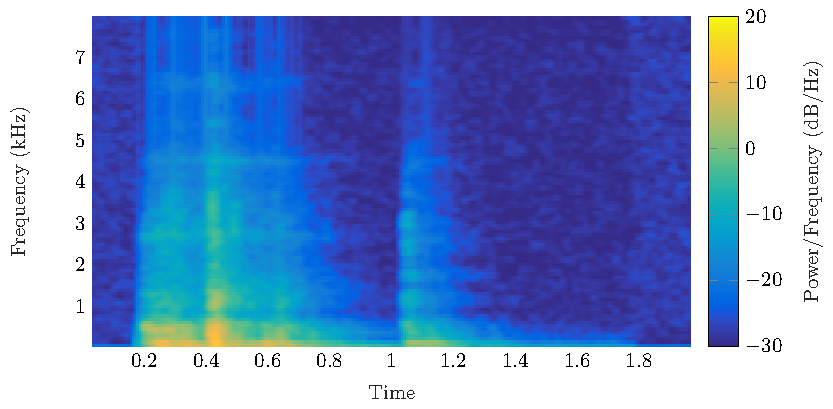
\includegraphics[width=\textwidth]{img/cin/rndy_freq_.pdf}
		\caption{Human fall signal in the frequency domain.}\label{fig:spec_hf}
	\end{subfigure}
	
	\begin{subfigure}[t]{0.5\columnwidth}
		\centering
		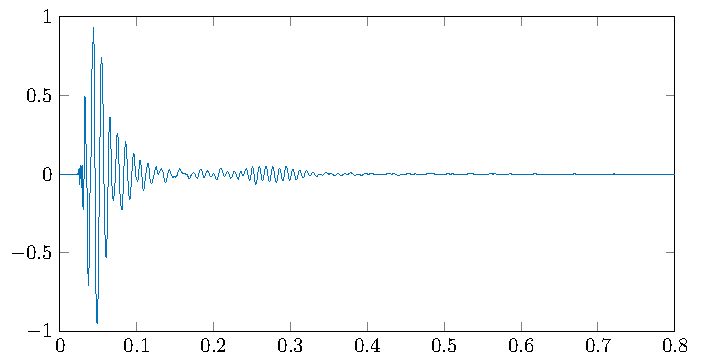
\includegraphics[width=0.9\textwidth]{img/cin/book_time_.pdf}
		\caption{Book fall signal in the time domain.}\label{fig:time_bf}
	\end{subfigure}%
	\begin{subfigure}[t]{0.5\columnwidth}
		\centering
		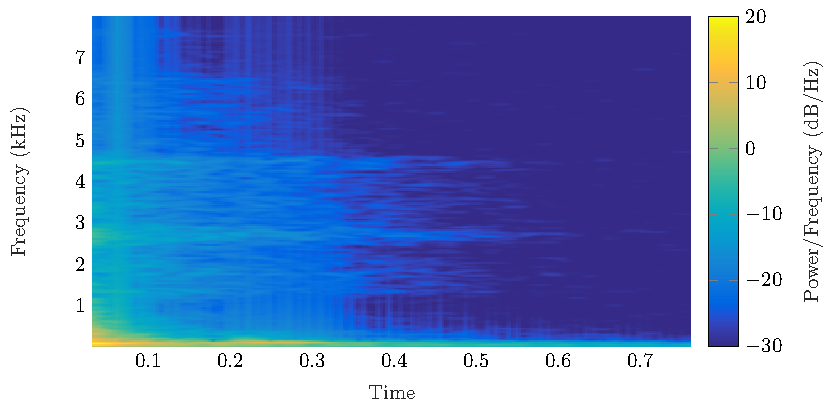
\includegraphics[width=\textwidth]{img/cin/book_freq_.pdf}
		\caption{Book fall signal in the frequency domain.}\label{fig:spec_bf}
	\end{subfigure}
	\caption{Time domain (on the left) and frequency domain (on the right) representation of a normal human activity signal (a-b), human fall signal (c-d), and book fall signal (e-f).}\label{fig:waveforms}
\end{figure}

The algorithm proposed in this paper reduces the problem by employing a multi-stage classification approach that combines a one-class classifier based on OCSVM with a template-matching stage. The OCSVM is trained unsupervisedly on a large corpus containing sounds that represent the ``normality''. On the contrary, the template-matching stage employs a set of templates represented by a small number of feature vectors marked as false alarm by the user. Thus, robustness against possible false alarms is achieved by using only few examples of false positive classes without the need of multiple sensors. An additional advantage with respect to the state of the art is that the proposed approach is able to evolve and improve after its initial training, since the template set can be augmented as non-falls events are detected.

\subsection{Proposed approach}
The proposed approach is composed of three stages \figref{fig:overall_ocsvm_user_aided}: the first (``Feature Extraction'') extracts MFCCs from the input audio signal and then GMSs to describe the entire audio segment. The second stage (``Abnormal Event Detection'') consists of a One-Class SVM classifier that discriminates between normal and abnormal sounds. Up to the authors' knowledge, OCSVM together with GMSs have never been jointly used for acoustic fall detection.  The third stage represents the innovative contribution of this paper for reducing false alarms in unsupervised approaches: it consists of a ``Template-Matching'' block that refines the output of the OCSVM and classifies the input data as fall or non-fall. The OCSVM is trained unsupervisedly on a large dataset of everyday sounds with the objective of discriminating normal from abnormal sounds. As aforementioned, the basic assumption is that the acoustic events related to human falls are ``rare'' respect to sounds normally occurring inside a home. The template-matching stage, on the other side, requires a set of ``template'' instances that represent rare events that can be confused with a fall. Referring to \figref{fig:overall_ocsvm_user_aided}, the ``Template-Matching'' stage is composed of a set of ``Templates'', a block that calculates the distance between the input GMS and the templates (``Euclidean Distance Calculation''), and a ``Decision'' block the decides whether the event is a fall or a non-fall by evaluating the magnitude of the distance.  The rationale here is that certain acoustic events are as abnormal as falls and confuse the OCSVM: the template-matching stage reduces false positives by using a set of examples related to the most confusing classes. In this work, the algorithm is ``user-aided'', i.e., templates are indicated by the user each time the OCSVM produces a false positive. This is shown in \figref{fig:overall_ocsvm_user_aided} with the person silhouette near the block that decides whether a detected fall is a false positive or not (``False Positive?''). In general, however, it is possible to create the templates set a-priori by recording several instances of possible false alarms events. Although rare, false alarm events (e.g., falls of objects) are certainly easier to reproduce in laboratory respect to human falls.

\subsubsection{Template Matching}
The template-matching classifier operates on a set of templates, i.e., supervectors, that can be defined a-priori or selected by the user when the OCSVM detects an abnormal sound that is not a human fall. Denoting with $\mathbf{x}$ the supervector of the input signal and with $\mathcal{Y} = \{\mathbf{y}_1,\ldots,\mathbf{y}_N\}$ the set of templates, the algorithm operates by calculating the Euclidean distance $D^{(i)} = \| \mathbf{x} - \mathbf{y}_i \|$ between the supervector to be classified and all the templates in the set. Indicating with $D_{min} = \underset{i}{\min}\,\,D^{(i)}$, the supervector $\mathbf{x}$ is classified as a fall if $D_{min}>\beta$ and as non-fall otherwise. The threshold $\beta$ is a hyperparameter of the algorithm that can be determined on a validation set.

\begin{figure}[t]
	\centering
	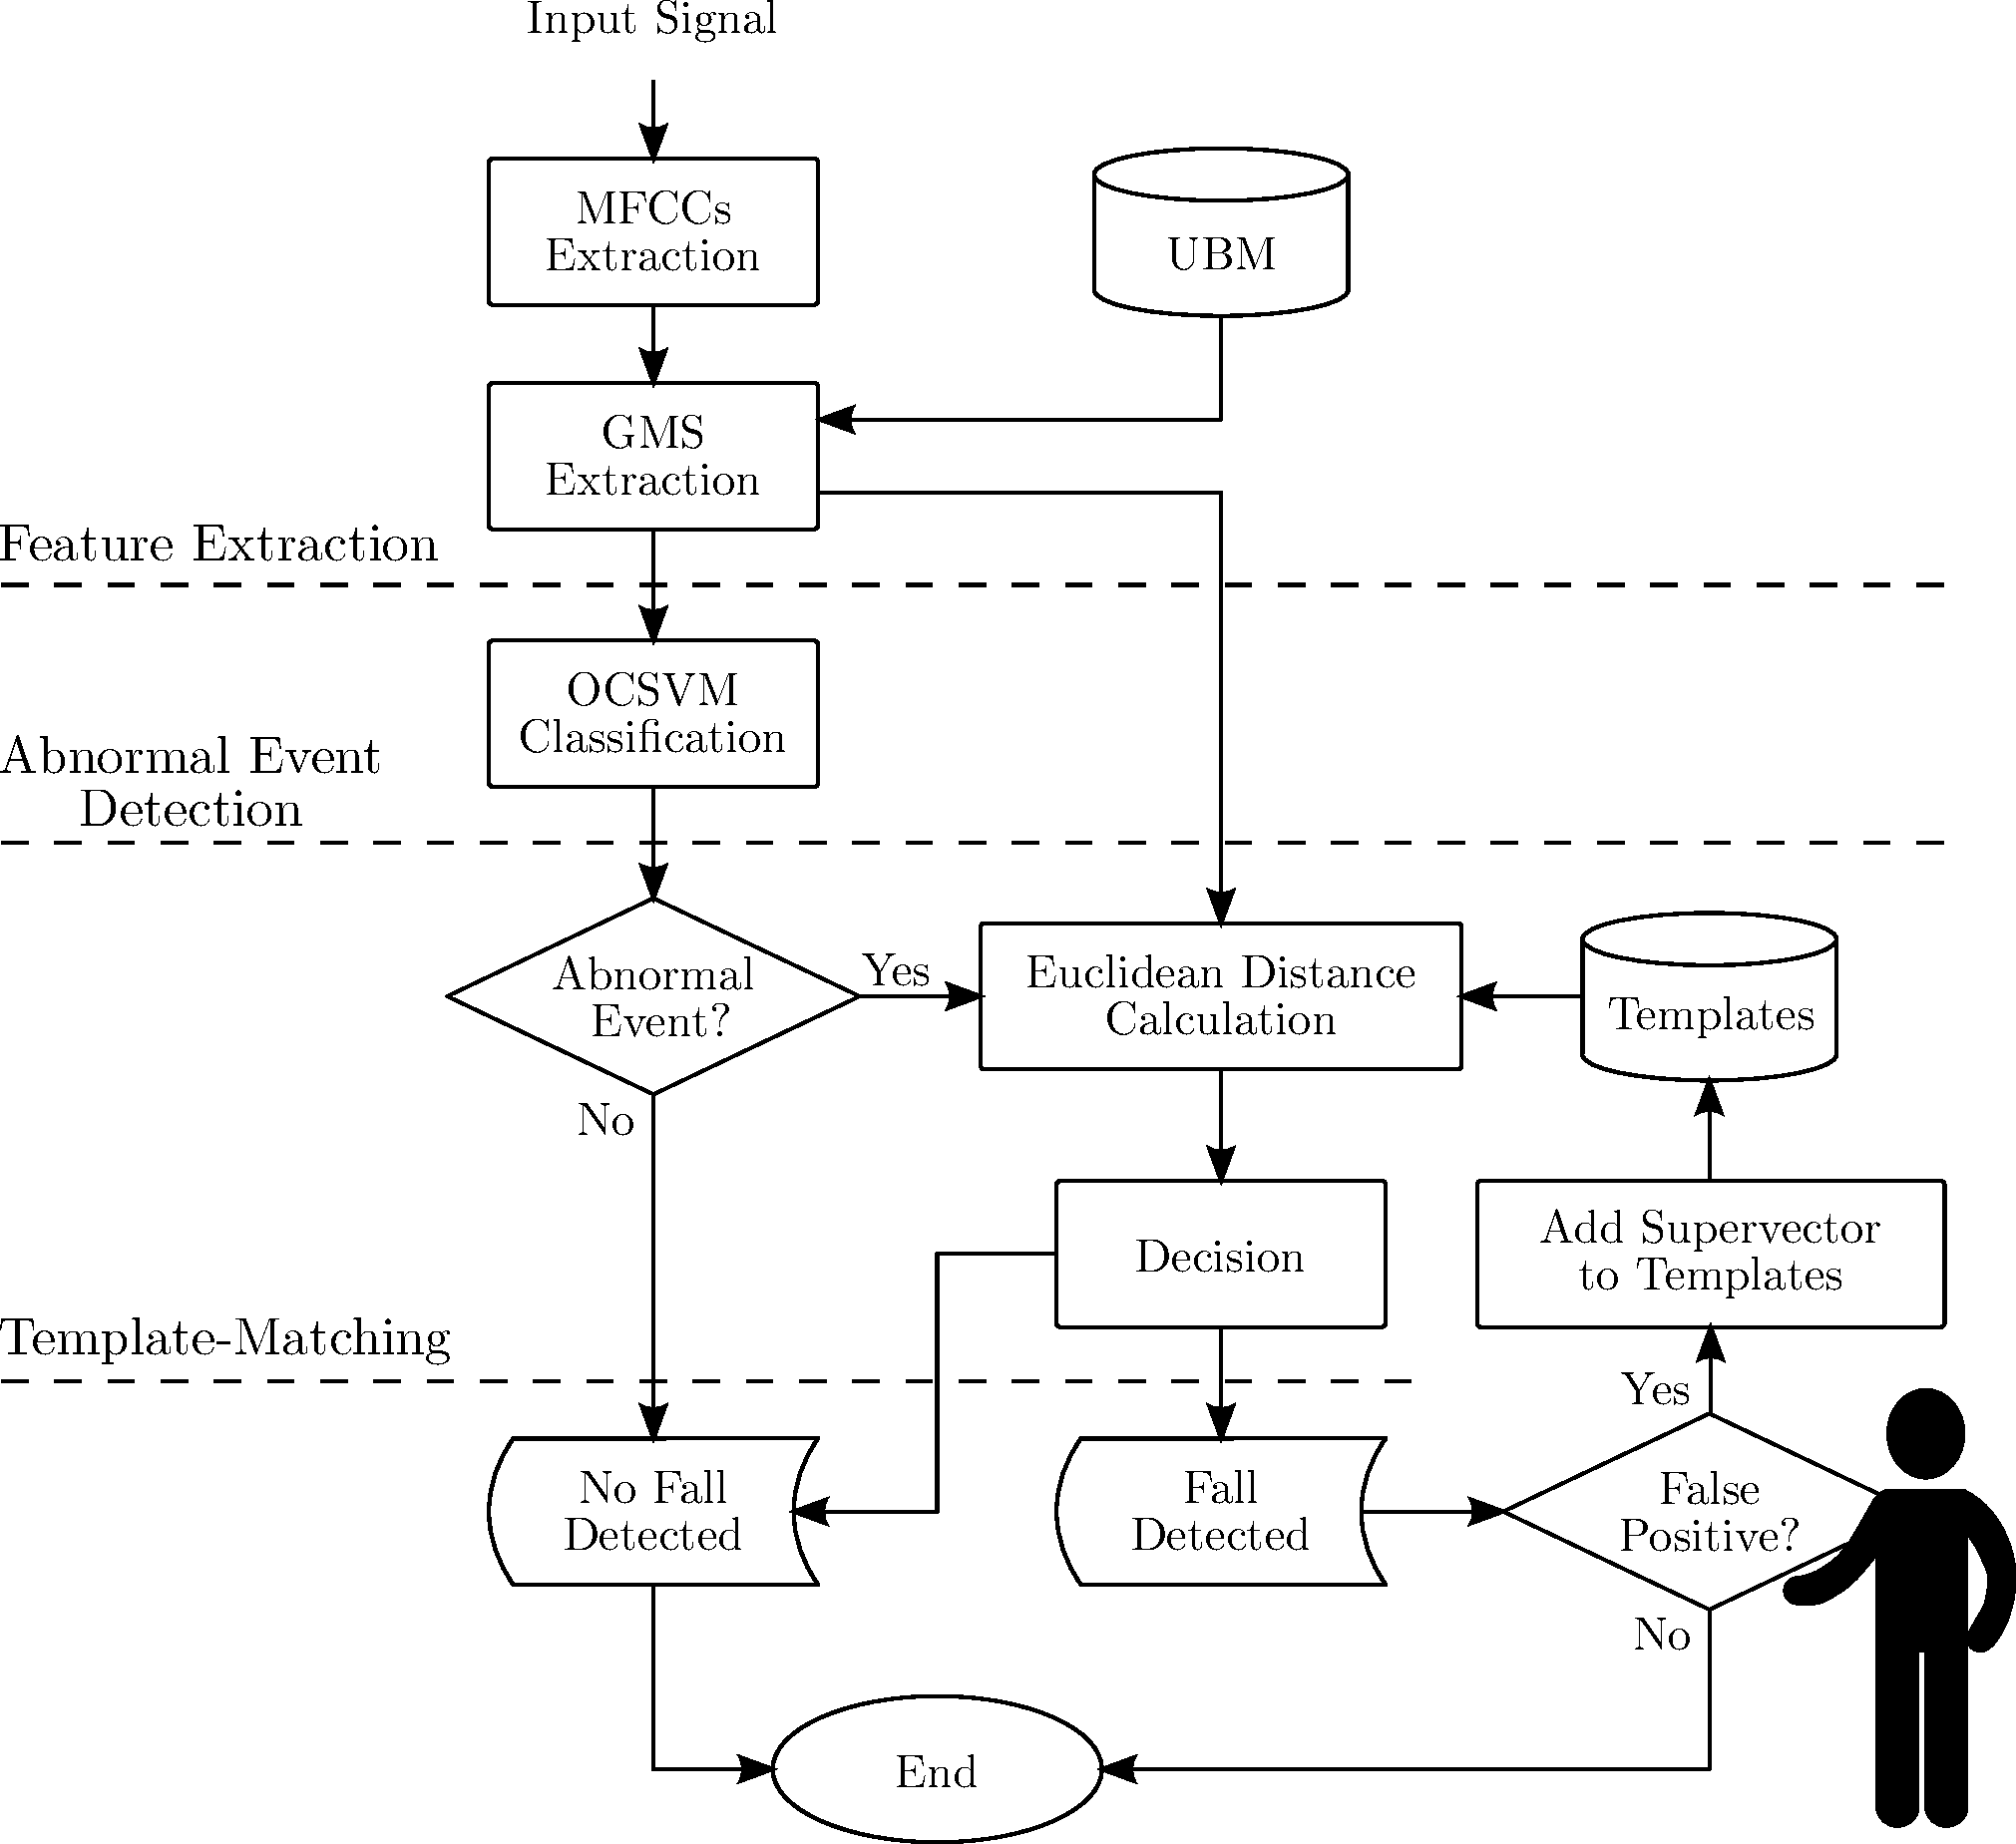
\includegraphics[width=0.95\columnwidth]{img/cin/approccioComplessivo.pdf}
	\caption{The block scheme of the proposed approach.}\label{fig:overall_ocsvm_user_aided}
\end{figure}

\subsection{Dataset}

The dataset employed in this method is the same used for the approach proposed in \secref{sec:ocsvm_approach} and reported in \tableref{tab:ocsvm_dataset}. Please refer to \secref{sec:dataset_cin_ocsvm_only} for the details.

\subsection{Experimental setup}
As in the system presented in \secref{sec:ocsvm_approach}, the dataset has been divided in one set for training the UBM and the OCSVM and three sets for evaluating the performance.
Training has been performed on the same set used for the OCSVM base algorithm presented in \secref{sec:ocsvm_approach} and shown in \tableref{tab:trainComposition}. The same three sets described in \secref{sec:experiment_ocsvm} has been used for the assessment and summarized below as a reminder:
\begin{itemize}
	\item Set 1: Human fall and background sounds (\tableref{tab:set1Composition_}).
	\item Set 2: Human fall and object fall sounds (\tableref{tab:set2Composition_}).
	\item Set 3: Human fall, object fall and background sounds (\tableref{tab:set3Composition_}).
\end{itemize}


\begin{table}[t]
	\centering
	\caption{Data used in ``Set 1''.}
	\begin{subtable}[t]{.6\textwidth}
		\centering		
		\caption{Composition  of ``Set 1''.}
		\label{tab:set1Composition_} % è lo stesso del capitolo 5. Lo riporto qui per comodità di lettura
		\begin{center}
			\begin{tabular}{K{3cm}K{3cm}}				
				\hline
				\textbf{Class} & \textbf{Nr.\ of occurrences} \\ 
				\hline
				$\,$ Human Falls $\,$ 	& 44    			\\
				Human Activity  		& 15		\\
				Music			  		& 29		\\
				%				 Classic Music       	& 15   		\\
				%				 Rock Music       		& 14  		\\		
				\hline
			\end{tabular}			
		\end{center}		
	\end{subtable}%
	\begin{subtable}[t]{.6\textwidth}
		\centering		
		\caption{Templates of ``Set 1''.}\label{tab:set1Template}
		\begin{center}
			\begin{tabular}{ccc}
				
				\hline
				\multirow{2}{1cm}{\textbf{Class}}	& \multicolumn{2}{c}{\textbf{Nr.\ of templates}}	\\ 
				\cline{2-3}
				&\textbf{Clean}&\textbf{Noisy}						\\
				%& \hspace{8pt}Clean\hspace{8pt}  & \hspace{6pt}Clean\hspace{6pt}   \\ 
				\hline
				Human Activity  		& 13	&	11 		\\
				Music       	& 8   	&	16		\\
				%				 Classic Music       	& 8   	&	16		\\
				%				 Rock Music       		& 0  	&	0		\\	
				\hline
				Total					& 21  	&	27		\\
				\hline
			\end{tabular}
			
		\end{center}
	\end{subtable}
	
	
\end{table}

\begin{table}[t]
	\centering
	\caption{Data used in ``Set 2''.}
	\begin{subtable}[t]{.6\textwidth}
		\centering
		
		\caption{Composition  of ``Set 2''.}
		\label{tab:set2Composition_}
		\begin{center}
			
			\begin{tabular}{K{3cm}K{3cm}}
				
				\hline
				\textbf{Class} & \textbf{Nr. of occurrences} \\ 
				%& \hspace{8pt}Clean\hspace{8pt}  & \hspace{6pt}Clean\hspace{6pt}   \\ 
				\hline
				$\,$ Human Falls $\,$ 	& 44    		\\				
				Basket      			& 7           	 \\
				Fork        			& 7           	 \\
				Ball       			& 8           	 \\
				Book        			& 7          	  \\
				Bag         			& 8          	  \\
				Chair       			& 7    			\\
				
				\hline
			\end{tabular}
			
		\end{center}
		
	\end{subtable}%
	\begin{subtable}[t]{.6\textwidth}
		\centering
		
		\caption{Templates of ``Set 2''.}
		\label{tab:set2Template}
		\begin{center}
			\begin{tabular}{ccc}
				
				\hline
				\multirow{2}{1cm}{\textbf{Class}}	& \multicolumn{2}{c}{\textbf{Nr.\ of templates}}	\\ 
				\cline{2-3}
				&\textbf{Clean}&\textbf{Noisy}						\\
				%& \hspace{8pt}Clean\hspace{8pt}  & \hspace{6pt}Clean\hspace{6pt}   \\ 
				\hline
				Basket  		& 55	&	57 		\\
				Fork       	& 39   	&	55		\\
				Ball      		& 11  	&	52		\\	
				Book  			& 26	&	57 		\\
				Bag       		& 26   	&	56		\\
				Chair       	& 86  	&	89		\\
				\hline	
				Total			& 243   &	366		\\	
				\hline
			\end{tabular}
			
		\end{center}
		
		
	\end{subtable}
	
	
\end{table}


\begin{table}[t]
	\centering
	\caption{Data used in ``Set 3''.}
	\begin{subtable}[t]{.6\textwidth}
		\centering
		
		\caption{Composition  of ``Set 3''.}
		\label{tab:set3Composition_}
		\begin{center}
			
			\begin{tabular}{K{3cm}K{3cm}}
				
				\hline
				\textbf{Class} & \textbf{Nr. of occurrences} \\ 
				%& \hspace{8pt}Clean\hspace{8pt}  & \hspace{6pt}Clean\hspace{6pt}   \\ 
				\hline
				$\,$ Human Falls $\,$ 	& 44    		\\				
				Basket      			& 3            	\\
				Fork        			& 4            	\\
				Ball       			& 4            	\\
				Book        			& 3            	\\
				Bag         			& 4            	\\
				Chair       			& 4    			\\
				Human Activity  		& 8   			\\
				Music			  		& 14   			\\
				%				 Classic Music       	& 7   			\\
				%				 Rock Music       		& 7   			\\
				
				\hline
			\end{tabular}
			
		\end{center}
		
	\end{subtable}%
	\begin{subtable}[t]{.6\textwidth}
		\centering
		
		\caption{Templates of ``Set 3''.}
		\label{tab:set3Template}
		\begin{center}
			\begin{tabular}{ccc}				
				\hline
				\multirow{2}{1cm}{\textbf{Class}}	& \multicolumn{2}{c}{\textbf{Nr.\ of templates}}	\\ 
				&\textbf{Clean}&\textbf{Noisy}						\\
				%& \hspace{8pt}Clean\hspace{8pt}  & \hspace{6pt}Clean\hspace{6pt}   \\ 
				\hline
				Basket      			& 52     &  57		\\
				Fork        			& 57     &  57 		\\
				Ball       			& 19     &  55  	\\
				Book        			& 53     &  57   	\\
				Bag         			& 50     &  56    	\\
				Chair       			& 89     &	89		\\
				Human Activity  	& 11   	 &	4		\\
				Music 			      	& 4   	 &	11		\\
				%							 Classic Music       	& 4   	 &	11		\\
				%							 Rock Music       		& 0   	 &	0		\\
				\hline	
				Total						& 335   &	386		\\	
				\hline
			\end{tabular}			
		\end{center}		
	\end{subtable}
	
	
\end{table}
The validation phase has been set following the same procedure described in section \secref{sec:experiment_ocsvm}: a cross-validation composed of four fold has been used for estimating the hyperparameter and  the final performance is calculated by using the cumulative true positives, false positives, and false negatives obtained by varying the test folds.
Differently from the previous method, the validation phase consisted not only in searching for the number of components of the UBM and the parameters ($\nu$ and $\gamma$) of the OCSVM, but also the value of the threshold $\beta$ in the template-matching stage. The values assumed by these variables are summarized in \tableref{tab:parameter}.
The method employed for the template-matching decision threshold is explained in \secref{ssec:templateThreshold}.

%\subsection{Comparative method}

\begin{table}[t]
	\centering
	\caption{Hyperparameters of the algorithm and search space explored in the validation phase. The search space of the template-matching threshold $\beta$ is not reported, since is determined with the procedure described in \secref{ssec:templateThreshold}. }
	\label{tab:parameter}
	\begin{tabular}{c |c | c}
		\hline
		\textbf{Stage} & \textbf{Hyperparameter} & \textbf{Range} \\
		\hline
		UBM & $J$ & $1, 2, 4, \ldots , 64$\\
		\hline
		\multirow{2}{*}{OCSVM} & $\nu$ & $0.1, 02, \ldots, 1.0$ \\
		&$\gamma$ & $2^{-15}, 2^{-13}, \ldots,2^{3} $ \\
		\hline
		Template-matching & $\beta$  & See \secref{ssec:templateThreshold}\\
		\hline
	\end{tabular}
\end{table}

All the aforementioned datasets require a set of templates for the template-matching stage of the algorithm. In the case of object falls, the set of templates has been created by classifying a set of 372 object falls with the OCSVM and selecting the occurrences misclassified as human falls. In the case of background sounds, the set of templates has been created by calculating the Euclidean distance between each occurrence of the development-set and each occurrence of a set of 470 background signals and then selecting the segment whose distance is minimum. Details on the templates sets are shown in \tableref{tab:set1Template}, \tableref{tab:set2Template}, and \tableref{tab:set3Template} respectively for ``Set 1'', ``Set 2'', and ``Set 3''.


The proposed approach has been compared with the method from which it derives (\secref{sec:ocsvm_approach}) and the algorithm presented in \cite{Popescu2009} based on OCSVM (please revert to \paragref{par:popescu_mod} for the details) 

The performance has been evaluated in terms of F$_1$-Measure \eqref{eq:f1} 

\subsection{Choice of the template-matching decision threshold}\label{ssec:templateThreshold}
A key point of the proposed approach is the decision threshold $\beta$ in the template-matching stage. Choosing a too low value would result in a low number of false negatives and a high number of false positives. On the contrary, a too high value would result in a high number of false negatives and a low number of false positives. The choice of $\beta$ has been performed by calculating the minimum Euclidean distance between each fall and non-fall event in the validation set and the set of templates. \figref{fig:distr_clean} and \figref{fig:distr_noisy} show respectively the probability distributions for the three sets in clean and noisy conditions. The decision threshold $\beta$ has been chosen at the intersection point between the distribution of fall and non-fall distances. This choice represents a compromise that balances false positives and false negatives.

Observing clean condition distributions, in ``Set 1'' the two density are considerably overlapped, while in ``Set 2'' the overlap is modest. It is expected that the possible improvement of the template-matching stage will be more consistent for ``Set 2'' respect to ``Set 1''. ``Set 3'' contains human activity and music occurrences as ``Set 1'' and object falls as ``Set 2'': indeed, the probability distributions (\figref{fig:distr_clean_set3}) are more distinct respect to the ones of ``Set 1'', but not so much as the ones of ``Set 2''.

Noisy condition distributions, shown in \figref{fig:distr_noisy}, are in general less distinct compared to clean condition ones. The effect of noisy is to flatten the distances of the fall and non-fall classes, thus resulting in a less discriminative capabilities of the classifier. Thus, it is expected that the performance improvement in noisy conditions will be more modest respect to the one obtained in clean condition.

\begin{figure}[t]
	\centering
	\begin{subfigure}{0.9\columnwidth}
		\centering
		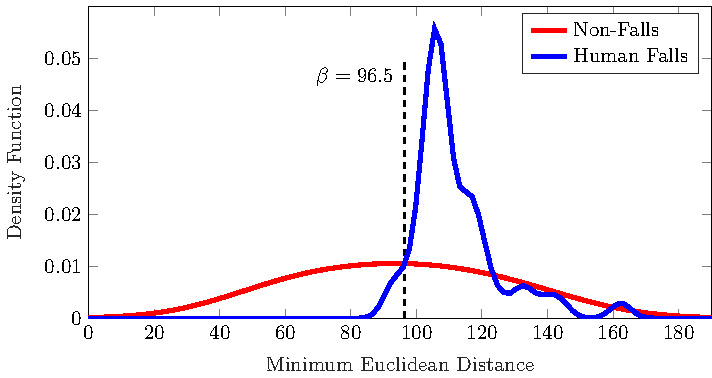
\includegraphics[width=0.98\columnwidth]{img/cin/distribuzione_Caso1_Clean.pdf}
		\subcaption{Probability distributions related to ``Set~1''.}\label{fig:distr_clean_set1}
	\end{subfigure}\hspace{1pt}
	\begin{subfigure}{0.9\columnwidth}
		\centering
		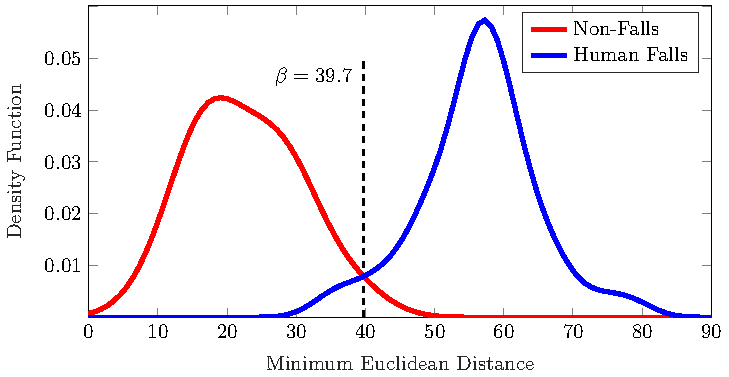
\includegraphics[width=\columnwidth]{img/cin/distribuzione_Caso2_Clean.pdf}
		\subcaption{Probability distributions related to ``Set~2''.}\label{fig:distr_clean_set2}
	\end{subfigure}\hspace{1pt}
	\begin{subfigure}{0.9\columnwidth}
		\centering
		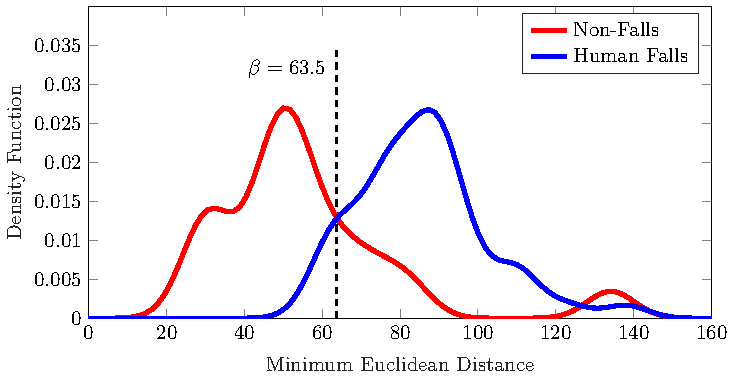
\includegraphics[width=\columnwidth]{img/cin/distribuzione_Caso3_Clean.pdf}
		\subcaption{Probability distributions related to ``Set~3''.}\label{fig:distr_clean_set3}
	\end{subfigure}
	\caption{Probability distributions of the minimum Euclidean distances among the template sets, and human falls and non-falls in \textit{clean} acoustic condition.}\label{fig:distr_clean}
\end{figure}

\begin{figure}[t]
	\centering
	\begin{subfigure}{0.9\columnwidth}
		\centering
		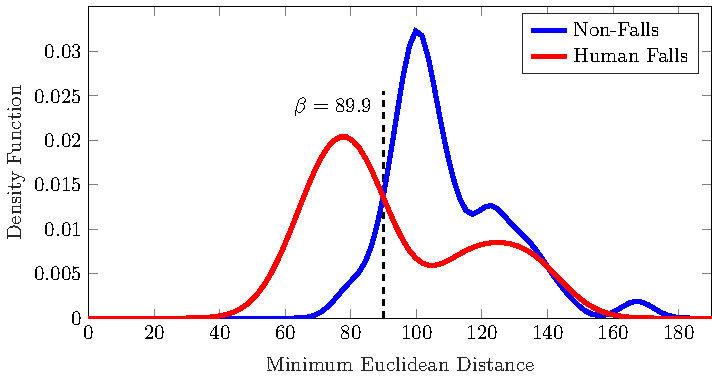
\includegraphics[width=0.98\columnwidth]{img/cin/distribuzione_Caso1_Noisy.pdf}
		\subcaption{Probability distributions related to ``Set~1''.}
	\end{subfigure}\hspace{1pt}
	\begin{subfigure}{0.9\columnwidth}
		\centering
		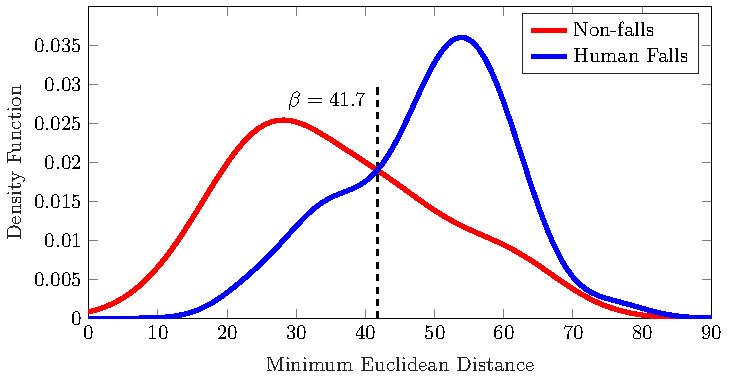
\includegraphics[width=\columnwidth]{img/cin/distribuzione_Caso2_Noisy.pdf}
		\subcaption{Probability distributions related to ``Set~2''.}
	\end{subfigure}\hspace{1pt}
	\begin{subfigure}{0.9\columnwidth}
		\centering
		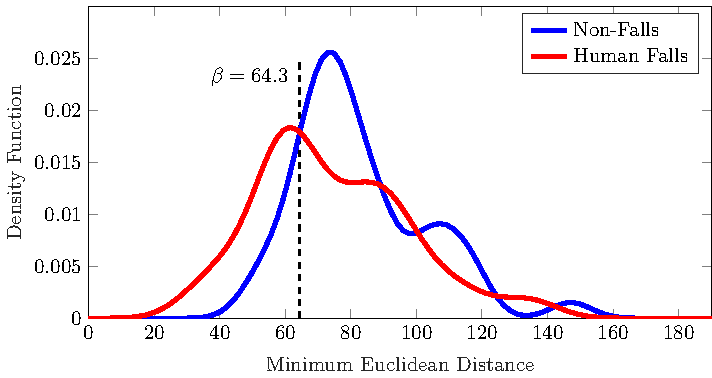
\includegraphics[width=\columnwidth]{img/cin/distribuzione_Caso3_Noisy.pdf}
		\subcaption{Probability distributions related to ``Set~3''.}
	\end{subfigure}%
	\caption{Probability distributions of the minimum Euclidean distances among the template sets, and human falls and non-falls in \textit{noisy} acoustic condition.}\label{fig:distr_noisy}
\end{figure}

\subsection{Results}
\figref{fig:res_clean_} shows the results in clean conditions obtained with and without the template-matching stage, respectively denoted as ``OCSVM+Template-Matching'' and ``OCSVM''. The results obtained with the method proposed in \cite{Popescu2009} are denoted with ``Popescu (2009)''. Observing the figure, it is evident that in all the three cases the template-matching approach is able to improve the performance with respect to ``Popescu (2009)'' \cite{Popescu2009} and the OCSVM only approach. In particular, in ``Set 1'', that comprises human falls, human activities and music, the performance improves by 2.03\% with respect to OCSVM and by 19.64\% with respect to ``Popescu (2009)''. This case can be considered as the least challenging of the three, since non-falls events are considerably different from falls ones. Conversely, ``Set 2'' comprises both human falls and object falls, thus it includes abnormal events whose pattern is similar to the one of human falls. The introduction of the template-matching stage considerably reduces the number of false positives, leading to an overall performance improvement of 20.76\%. ``Set 3'' comprises human falls, human activities, music and object falls and represents the most realistic test condition of the three. Introducing the template-matching stage, the performance improves by 7.64\%, leading to an F$_1$-Measure equal to 89.89\%. 

\begin{figure}[t]
	\centering
	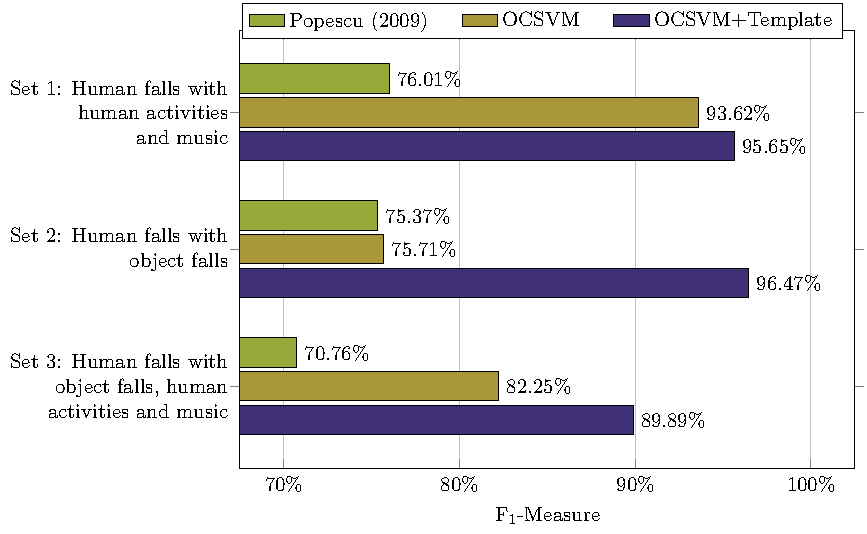
\includegraphics[width=\columnwidth]{img/cin/res_clean.pdf}
	\caption{Results in \textit{clean} conditions for the three test cases. ``Set 1'' comprises human falls, human activities and music. ``Set 2'' comprises human falls and object falls. ``Set 3'' comprises human falls, object falls, human activities, and music.} \label{fig:res_clean_}
\end{figure}

\figref{fig:res_noisy_} shows the results obtained for the three cases in noisy conditions. As expected, the performance decreases in all the three evaluated methods. In ``Set 1'', the performance decrease is modest (2.32\% for the OCSVM, 2.63\% for the proposed approach, and 1.44\% for ``Popescu (2009)''), demonstrating that the OCSVM is able to effectively reject non-fall events corrupted by music interference. The use of the template-matching stage increases the performance by 1.72\%, thus providing a significant improvement also in noisy conditions. In ``Set 2'', Template-matching provides a performance improvement of 8.02\% with respect to the OCSVM, leading to an F$_1$-Measure higher than 70\%. The improvement is lower with respect to the clean ``Set 2'', since the variability of the music interference makes the Euclidean distances of fall and non-fall classes more similar and is not sufficient to overcome the ``Popescu (2009)'' \cite{Popescu2009}. In ``Set 3'', the proposed approach improves the performance by 4.77\% with respect to OCSVM and by 8.68\% with respect to ``Popescu (2009)''.

In summary, the results demonstrated that the introduction of a template-matching stage significantly improves the performance both of the OCSVM only approach and of the method by Popescu and Mahnot \cite{Popescu2009}: averaging the results over ``Set 1'', ``Set 2'', and ``Set 3'', the absolute improvement with respect to the former is 10.14\% in clean conditions and 4.84\% in noisy conditions. With respect to the latter \cite{Popescu2009} the improvement is 19.96\% in clean conditions and 8.08\% in noisy conditions. As shown in \figref{fig:res_clean_} and \figref{fig:res_noisy_}, both in clean and noisy conditions the F$_1$-Measure of the method by Popescu and Mahnot \cite{Popescu2009} is close to 75\% in ``Set 1'' and ``Set 2'', and close to 71\% in ``Set 3''. The different behaviour compared to the OCSVM only approach can be attributed firstly to the different feature representation of the audio signal (MFCCs instead of supervectors). Secondly, to the strategy adopted for classification: in \cite{Popescu2009}, signals are divided in windows and a fall is detected if at least two consecutive windows are classified as fall. Differently, in the proposed algorithm, the overall signal is represented by a single supervector and classified as fall or non fall.

Comparing the results in clean (\figref{fig:res_clean_}) and noisy (\figref{fig:res_noisy_}) conditions, it is evident that techniques for reducing the impact of additive noise are needed. Additionally, the proposed solution requires the intervention of the user for selecting the templates after the first classification stage performed by the OCSVM. This aspect will be addressed in next sections in order to make the algorithm completely independent of the user, using a low number of examples related to human fall.

\begin{figure}[t]
	\centering
	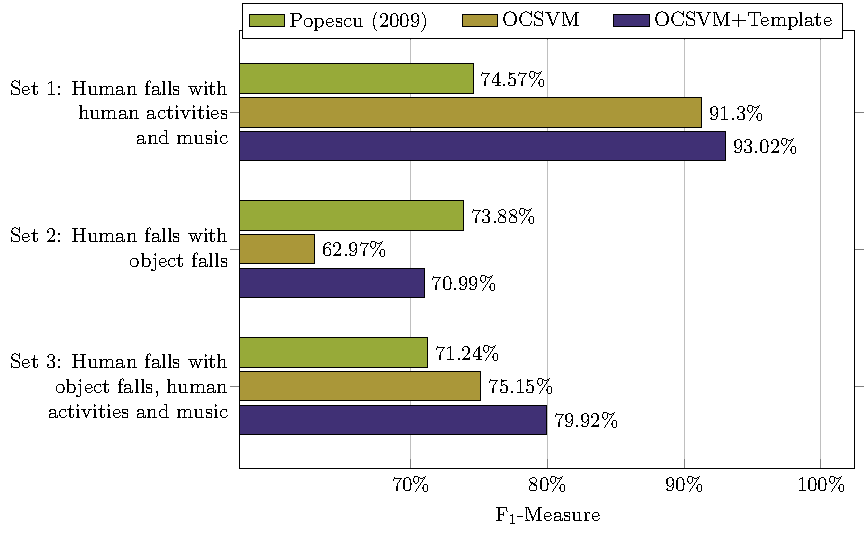
\includegraphics[width=\columnwidth]{img/cin/res_noisy.pdf}
	\caption{Results in noisy conditions for the three test cases. ``Set 1'' comprises human falls, human activities and music. ``Set 2'' comprises human falls and object falls. ``Set 3'' comprises human falls, object falls, human activities, and music.} \label{fig:res_noisy_}
\end{figure}
\section{Few-shot Siamese Neural Networks employing Audio features
for Human-Fall Detection}
\label{sec:siamese_few_shot}
\section{Audio Metric Learning by using Siamese Autoencoders
for One-Shot Human Fall Detection}
\label{sec:siamese_one_shot}